\section{Проектування системи}
\subsection{Розробка вимог до програмної системи}
\subsubsection{Функціональні вимоги} \label{section:requirements_functional}
Специфікацію функціональних вимог у вигляді \acrshort{uml}-діаграми прецедентів представлено на рисунку~\ref{fig:my_usecase}.
\begin{figure}[H]
    \centering
    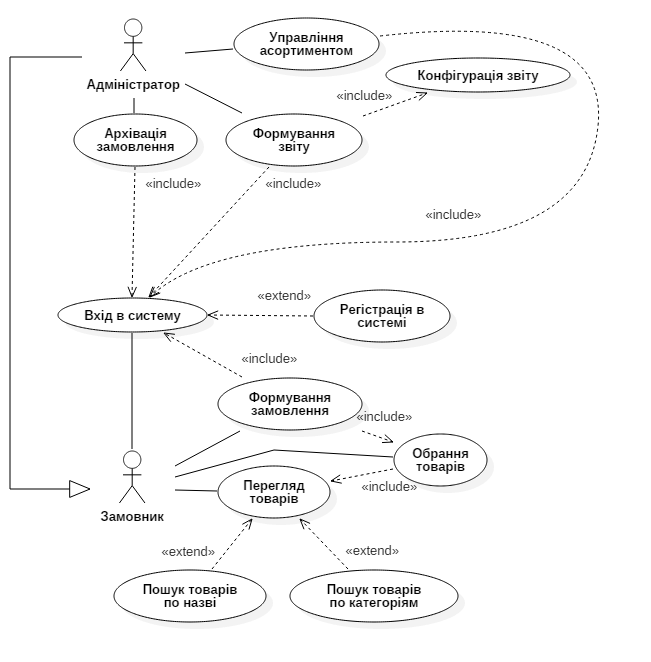
\includegraphics[width=0.8\textwidth]{my_usecase}
    \caption{Прецеденти системи в \acrshort{uml}-нотації}
    \label{fig:my_usecase}
\end{figure}

Управління асортиментом включає в себе можливість додавання нових категорій товарів, новий товарів, редагування інформації по старим товарам, видалення товарів та категорій товарів.

За записами в архіві можливе формування звітів. 

Звіт повинен мати наступну інформацію:
\begin{itemize}
    \item номер замовлення;
    \item дату замовлення і дату надсилання в архів;
    \item назви замовлених товарів (з визначенням категорії товару), їх кількість та ціну;
    \item загальну вартість замовлення.
\end{itemize}

Конфігурація формування звіту передбачає фільтрацію замовлень за датою замовлення, датою надсилання в архів, назвою товару, його категорією, кількістю товару, загальною вартістю замовлення. 

\subsubsection{Нефункціональні вимоги}
Список нефункціональних вимог системи:
\begin{enumerate}[label=\arabic*)]
    \item система повинна бути легко розширювана додатковим функціоналом;
    \item система повинна бути розрахована на 100 запитів у секунду та 10000 користувачів;
    \item система повинна не допускати можливості викрадення приватних даних користувачів.
\end{enumerate}

\subsection{Розробка концептуальної моделі даних}
На концептуальному рівні представлення даних інформація про деяку \acrshort{domain} представляється у вигляді її моделі даних без урахування будь-яких особливостей її подальшої комп'ютерної реалізації.

Концептуальна модель предметної області <<Інтернет магазин>> в нотації \acrshort{er} наведена на рисунку~\ref{fig:my_db_conceptual}.

\begin{figure}[H]
    \centering
    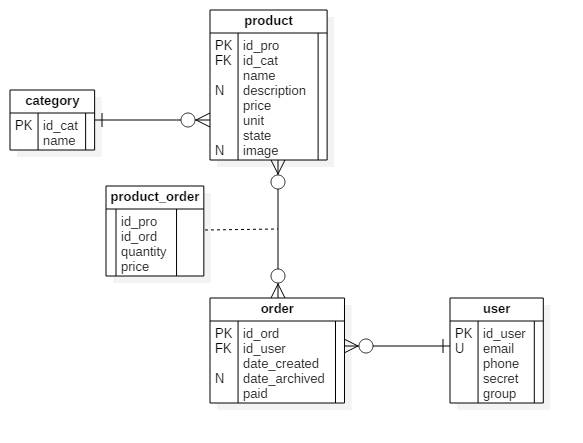
\includegraphics[width=0.8\textwidth]{my_db_conceptual}
    \caption{Концептуальна модель даних в \acrshort{er}-нотації}
    \label{fig:my_db_conceptual}
\end{figure}
\begin{description}
    \item[де] \texttt{category} --- категорія продуктів;
    \item \texttt{product} --- продукт;
    \item \texttt{user} --- користувач/адміністратор сайту.
    \item \texttt{order} --- замовлення продуктів.
    \item \texttt{product\_order} --- асоціативна сутність.
\end{description}

\subsection{Функціональна модель сайту}
Функціональна модель процесу замовлення товару на сайті представлена на рисунках~\ref{fig:my_idef0_1} та~\ref{fig:my_idef0_2}.
\begin{figure}[H]
    \centering
    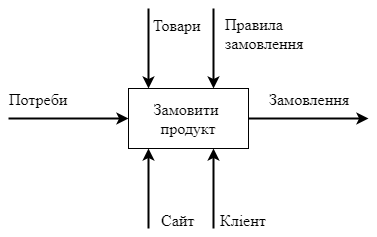
\includegraphics[width=0.6\textwidth]{my_idef0_1}
    \caption{Функціональна модель процесу замовлення товару (контекстний рівень)}
    \label{fig:my_idef0_1}
\end{figure}
\begin{figure}[H]
    \centering 
    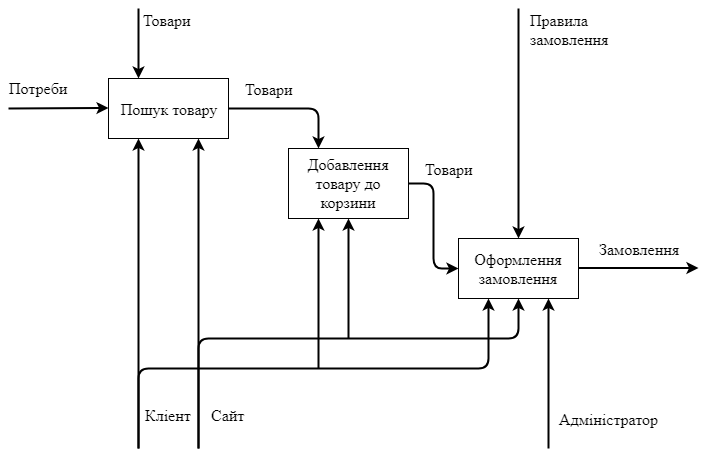
\includegraphics[width=\textwidth]{my_idef0_2}
    \caption{Функціональна модель процесу замовлення товару}
    \label{fig:my_idef0_2}
\end{figure}

Функціональна модель додавання товарів на сайт адміністратором представлена на рисунках~\ref{fig:my_idef0_add_product_1} та~\ref{fig:my_idef0_add_product_2}.
\begin{figure}[H]
    \centering
    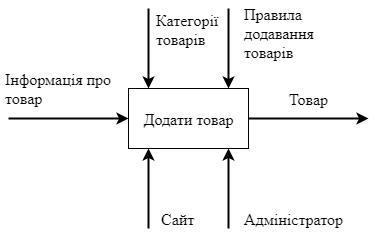
\includegraphics[width=0.6\textwidth]{my_idef0_add_product_1}
    \caption{Функціональна модель процесу додавання товарів на сайт (контекстний рівень)}
    \label{fig:my_idef0_add_product_1}
\end{figure}
\begin{figure}[H]
    \centering 
    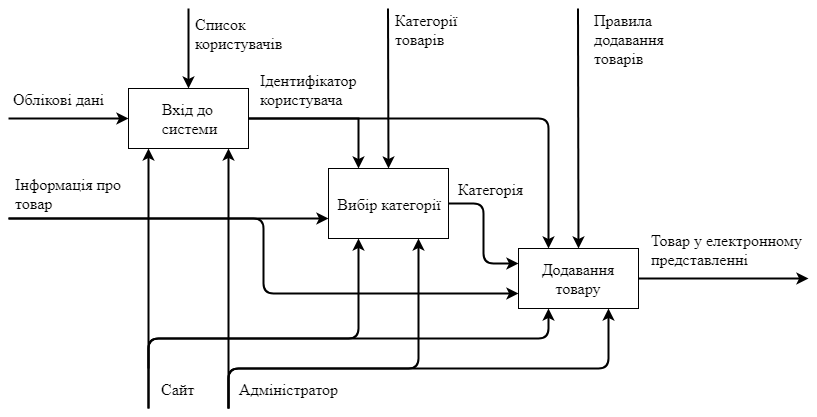
\includegraphics[width=\textwidth]{my_idef0_add_product_2}
    \caption{Функціональна модель процесу додавання товарів на сайт}
    \label{fig:my_idef0_add_product_2}
\end{figure}

\subsection{Обґрунтування вибору \acrshort{dbms} та інструментальних засобів}

\subsubsection{База даних SQLite}
SQLite --- це вбудована реляційна база даних, що поставляється з вихідними кодами.
Призначена для надання звичних можливостей реляційних баз даних без властивих їм накладних витрат.
За час експлуатації встигла заслужити репутацію як переносима, легка у використанні, компактна, продуктивна і надійна база даних\cite{SQLite2006a}.

\subsubsection{Apache \acrshort{http}-сервер}
Apache \acrshort{http}-сервер --- відкритий веб-сервер Інтернет для UNIX-подібних, Microsoft Windows, Novell NetWare та інших операційних систем.

Apache розроблюється та підтримується спільнотою розробників відкритого програмного забезпечення під керівництвом Apache Software Foundation~\cite{ApacheServer}.

\subsubsection{Текстовий редактор Sublime Text}
Sublime Text --- швидкий платформонезалежний редактор вихідних кодів програм.
Особливостями редактору є виділення стовпців і множинна правка, авто-доповнення, підтримка систем збірки, перехід по файлам~\cite{SublimeText}.

\subsubsection{Система управління версіями Git}
Використання системи контролю версії є необхідним для роботи над великими проектами.

Система контролю дозволяє зберігати попередні версії файлів та завантажувати їх за потребою. 
Вона зберігає повну інформацію про версію кожного з файлів, а також повну структуру проекту на всіх стадіях розробки.

Git --- розподілена система керування версіями файлів та спільної роботи.
Git є однією з найефективніших, надійних і високопродуктивних систем керування версіями, що надає гнучкі засоби нелінійної розробки, що базуються на відгалуженні і злитті гілок~\cite{Chacon2009}.
